\section{Theorie}

\subsection{Übersicht}
\begin{frame}{Übersicht}
	\begin{center}
		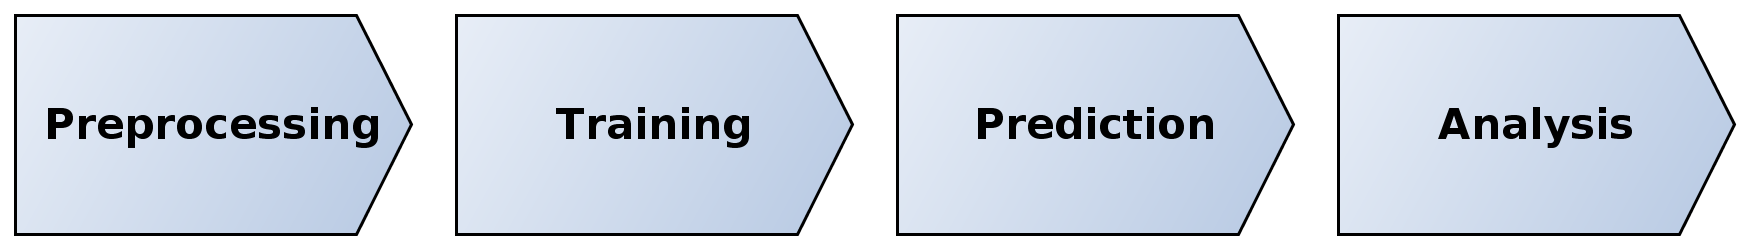
\includegraphics[width=1.0\textwidth]{img/theorieuebersicht}
	\end{center}
\end{frame}

\subsection{Ablauf}
\begin{frame}{Preprocessing}
	\begin{itemize}[<+->]
		\item Konvertierung des Audiosignals
		\begin{itemize}[<1->]
			\item Mono
			\item 16000 Hz
			\item 16 Bit
		\end{itemize}
		\item Feature Extraction
		\begin{itemize}[<1->]
			\item Linear Predictive Coding (LPC)
			\item Mel Frequency Cepstral Coefficients (MFCC)
		\end{itemize}		
		\item Skalierung
	\end{itemize}
\end{frame}

\begin{frame}{Training}
	\begin{columns}
	\column{0.65\linewidth}
		\begin{itemize}[<+->]
			\item Neural Gas
			\begin{itemize}[<1->]
				\item Robustes Neuronales Netz
				\item Nachbarschaftsreichweite
				\item $\begin{aligned}[t]\Delta w_{i} = \epsilon(t) * e^{\left(-k_i / \lambda(t)\right)} * \left(x - w_i\right)\end{aligned}$
			\end{itemize}
			\item Support Vector Machine (SVM)
			\begin{itemize}[<1->]
				\item Optimaler Klassifikator
				\item Multi-Class SVM
			\end{itemize}
		\end{itemize}
		\column{0.35\linewidth}
		\begin{center}
			\includegraphics<1>[width=1.0\textwidth]{img/neuralGas}
			\includegraphics<2>[width=1.0\textwidth]{img/svm}
		\end{center} 
	\end{columns}
\end{frame}

\begin{frame}{Prediction}
	\begin{itemize}[<+->]
		\item Nearest Neighbor
		\begin{itemize}[<1->]
			\item Distanz zwischen Eingabevektor und Codebookvektoren
		\end{itemize}
		\item Klassifikation
	\end{itemize}
\end{frame}

\begin{frame}{Analysis}
	\begin{itemize}[<+->]
		\item Erkennungsrate auf Einzelframes
		\item Erkennungsrate auf mehreren Frames
		\item Verwechslungsmatrix
	\end{itemize}
\end{frame}
